\chapter{State of the Art}

In this chapter we will explain the current state of computer graphics its latest advances and how ray tracing fits into it. We will also be looking at the technologies being used in both research and industry. 

% Explain basis of ray tracing and how it compares against rasterization
\section{Rendering Techniques}
The field of computer graphics seeks to generate images with the aid of computers. Nowadays this is a core component of photography, film production and videogames among others. This task is commonly refered to as \textit{rendering}. Throughout the years there have appeared many rendering techniques, of which the main ones being used currently are Rasterization and Ray Tracing.

\subsection{Rasterization}
Rasterization is the process of taking an image described as vector graphics and converting it into a series of pixels which, when displayed together, recreate the image that was represented with vector shapes. This image can then be displayed in a monitor, stored as a bit map and so on.

In figure \ref{rasterization-triangle-image}, from \cite{ScratchPixel} we see the principle of this process. After transforming the geometry (in this case a triangle) to screen space, we check if each pixel in the image overlaps said geometry.

\begin{figure}[hbt!]
    \centering
    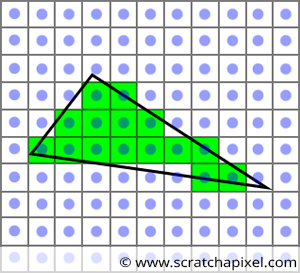
\includegraphics[width=0.6\textwidth]{figuras/rasterization-triangle1.png}
    \caption{Image being rasterized into pixels, extracted from \href{https://www.scratchapixel.com/lessons/3d-basic-rendering/rasterization-practical-implementation/rasterization-stage}{ScratchPixel}}
    \label{rasterization-triangle-image}
\end{figure}
When compared to other techniques for rendering 3D models, such as ray tracing, rasterization is extremely fast. This gives it a prevalent usage in real time 3D engines. We must take into account that the process of rasterization is only responsible for mapping the scene geometry to pixels, and does not compute the color of such pixels. This color is assigned by a Pixel (or Fragment) Shader, which is completely programmable in modern GPUs. This shader may take into account physical processes like light position, or a purely artistic approach. There is no motivation in modifying the rasterization techniques at render time. Therefore, the rest of the process of rasterizing a 3D model into screen space (a 2D plane for displaying said graphics) is often performed by non-programmable hardware with a fixed function within the graphics pipeline. This method allows for high efficiency.

\subsection{Ray Tracing}
The other prevalent technique for drawing 3D graphics, and the main focus of this work, is ray tracing.

This technique models light transport for generating digital images. It does this tracing a path from an imaginary eye through each pixel in a virtual screen and calculating the color of the object visible through it. Each ray is tested for intersection with some subset of the objects in the scene. Once identified the object, it estimates the incoming light at the intersection point and read the material properties of the object to calculate the final color of the pixel.

Although counter intuitive, sending rays \textit{from} the camera towards the scene is many orders of magnitude more efficient than doing it the other way around. This is due to the vast majority of rays coming from a light source not reaching the viewer's eye, thus saving a lot of computation in paths that are never recorded. We take the shortcut of assuming that a given ray intersects the view frame. After a certain number of reflections or distance traveled by a ray without intersecting anything, that ray ceases to travel and the pixel's value is updated. Figure \ref{rt-overview-image} shows an overview of this algorithm extracted from the Wikimedia \cite{WikimediaRT}.


\begin{figure}[hbt!]
    \centering
    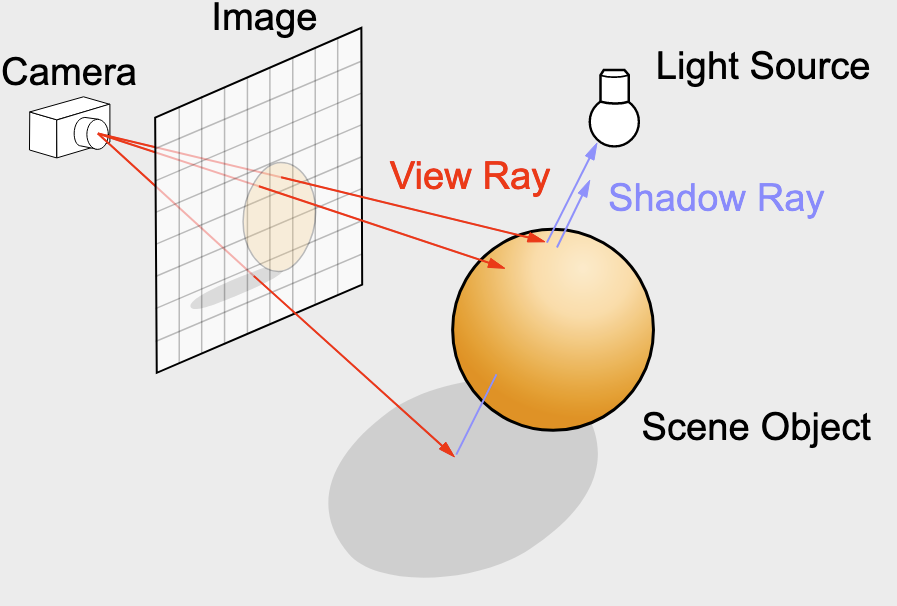
\includegraphics[width=1.0\textwidth]{figuras/RT-Diagram.png}
    \caption{Overview of the ray tracing algorithm with spheres as our only geometry and a single light source.}
    \label{rt-overview-image}
\end{figure}

Compared to rasterizing, all the techniques based in ray tracing are generally slower yet provide higher fidelity results than it's counterpart. This made it so that originally it was applied in tasks that could tolerate a relatively long render time, such as film production or still image generation. Applications where rendering speed is critical, like videogames, were less suited for these algorithms. However, since 2018, real time ray tracing has become more feasible thanks to hardware acceleration becoming standard in commercial graphics cards.

\subsubsection{Mathematical foundation}
We will now look at the mathematical definition of ray tracing applied to a rectangular viewport, which is the focus area of this work.

Our inputs are:
\begin{itemize}
  \item[*]{An eye position $E \in \mathbb{R}^3$}
  \item[*]{A target position $T \in \mathbb{R}^3$}
  \item[*]{A field of view $\theta \in [0, \pi]$. For humans, we can assume it's about 90 degrees ($\approx \frac{\pi}{2} radians $)}
  \item[*]{The number of square pixels in the vertical and horizontal directions in the viewport $m, k \in \mathbb{N}$}
  \item[*]{The actual number of pixels $i, j \in \mathbb{N}, 1 \leq i \leq k \land 1 \leq j \leq m$}
  \item[*]{A vertical vector that indicates the up and down direction $\overrightarrow{v} \in \mathbb{R}^3$. Usually $\overrightarrow{v} = [0, 1, 0]$ (the roll component determines the viewport's rotation around it's center $C$, where the axis is the $ET$ rotation).}
\end{itemize}

We can see an illustration of these components in figure \ref{RaysViewportSchema}, extracted from the Ray Tracing Wikipedia article \cite{WikipediaRT}.

\begin{figure}[hbt!]
    \centering
    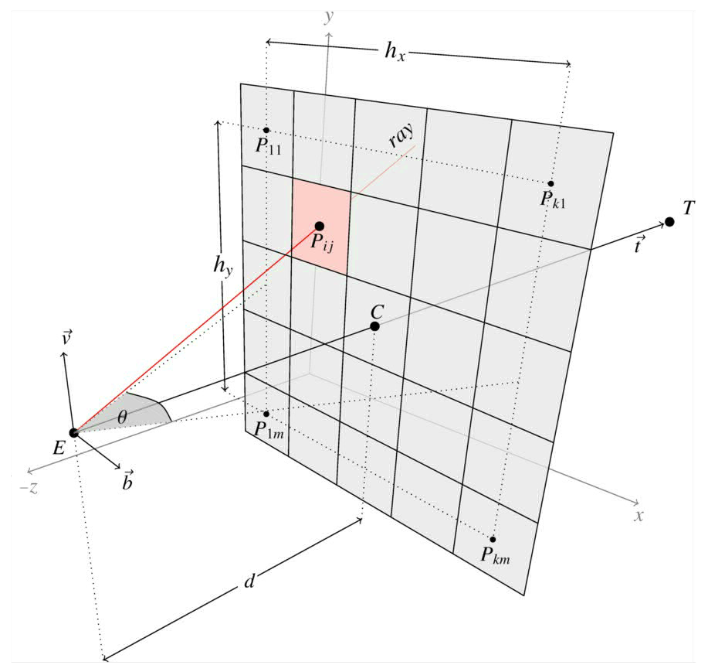
\includegraphics[width=1.0\textwidth]{figuras/RaysViewportSchema.png}
    \caption{Ray tracing schema with all the input components.}
    \label{RaysViewportSchema}
\end{figure}

With these inputs, our goal is to find the position of the center of each viewport pixel $P_{ij}$. This will allow us to find the line going from the eye $E$ through that pixel, and describe that ray by the point $E$ and the vector $\overrightarrow{R}_{ij} = P_{ij} - E$ (or its normalization $\overrightarrow{r}_{ij}$).

We start by finding the coordinates of the bottom left viewport pixel $P_{1m}$, and the subsequent ones by shifting along the directions paralell to the viewport (vectors $\overrightarrow{b}_{n}$ and $\overrightarrow{v}_{n}$), multiplied by the pixel size. The equations below include a distance $d$ between the eye $E$ and the viewport. This value will be reduced when normalizing the rays $\overrightarrow{r}_{ij}$, and as such can be interpreted as $d=1$ and removed from the calculations.

As a pre-calculation we normalize the vectors $\overrightarrow{t}$, $\overrightarrow{b}$ and $\overrightarrow{v}$, shown in figure \ref{RaysViewportSchema}, which are paralell to the viewport. This process is explained in equations \ref{eq-t-b}, \ref{eq-tn-bn} and \ref{eq-vn}.

\begin{equation}
  \overrightarrow{t} = T - E
  \text{,}
  \overrightarrow{b} = \overrightarrow{t} \times \overrightarrow{v}
  \label{eq-t-b}
\end{equation}

\begin{equation}
  \overrightarrow{t}_{n} = \frac{\overrightarrow{t}}{\left\Vert \overrightarrow{t} \right\Vert}
  \text{,}
  \overrightarrow{b}_{n} = \frac{\overrightarrow{b}}{\left\Vert \overrightarrow{b} \right\Vert}
  \label{eq-tn-bn}
\end{equation}

\begin{equation}
  \overrightarrow{v}_{n} = \overrightarrow{t}_{n} \times \overrightarrow{b}_{n}
  \label{eq-vn}
\end{equation}

Note that the viewport center is $C = E + \overrightarrow{t}_{n}d$.

We then calculate the viewport sizes $h_x$ and $h_y$, divided by $2$ including the inverse aspect ratio $\frac{m-1}{k-1}$. This is done in equation \ref{eq-g}.

\begin{equation}
  g_x = \frac{h_x}{2} = d * tan \frac{\theta}{2}
  \text{,}
  g_y = \frac{h_y}{2} = g_x \frac{m-1}{k-1}
  \label{eq-g}
\end{equation}

Next, we calculate the vectors used for shifting to the next pixel, $q_x$ and $q_y$, along the directions paralell to the viewport $\overrightarrow{b}$ and $\overrightarrow{v}$, from the bottom left pixel $p_{1m}$. This is shown in equations \ref{eq-q} and \ref{eq-p}.

\begin{equation}
  \overrightarrow{q}_x = \frac{2g_x}{k-1} \overrightarrow{b}_n
  \text{,}
  \overrightarrow{q}_y = \frac{2g_y}{m-1} \overrightarrow{v}_n
  \label{eq-q}
\end{equation}

\begin{equation}
  \overrightarrow{p}_{1m} = \overrightarrow{t}_n d - g_x \overrightarrow{b}_n - g_y \overrightarrow{v}_n
  \label{eq-p}
\end{equation}

If we consider $P_{ij} = E + \overrightarrow{p}_{ij}$ and the ray $\overrightarrow{R}_{ij} = P_{ij} - E = \overrightarrow{p}_{ij}$, we get the normalized rays in equation \ref{eq-r}.

\begin{equation}
  \overrightarrow{p}_{ij} = \overrightarrow{p}_{1m} + \overrightarrow{q}_x(i - 1) + \overrightarrow{q}_y(j - 1)
  \text{,}
  \overrightarrow{r}_{ij} = \frac{\overrightarrow{R}_{ij}}{\left\Vert \overrightarrow{R}_{ij} \right\Vert} = \frac{\overrightarrow{p}_{ij}}{\left\Vert \overrightarrow{p}_{ij} \right\Vert}
  \label{eq-r}
\end{equation}

% Introduce Vulkan and OptiX: main features, current real world usage, API organization, etc.
\section{Ray Tracing Technologies}
As previously said, though the ray tracing technique has existed for several decades now, it is only in recent years that GPU acceleration has made it usable for real time applications. This acceleration comes from one of several libraries or rendering APIs that offer the programmer a quick and easy way to interact with the graphics card.

It's also worth mentioning that we could technically develop a GPU-accelerated ray tracer with any rendering library from the last two decades, since anything that gives us control over the GPU could be used for parallelizing the required operations and give us a considerable speed increase. An example of this would be the Compute Shaders in OpenGL, which could process an image that we could then draw to a texture in screen made of two triangles. However, we will only be looking at libraries that include functionality exclusively dedicated to ray tracing.

Some of these libraries have legacies that extend to the era of rasterized-only graphics, while others were made from the ground up just for ray tracing. At the same time, each of them was designed with a specific use case in mind, be it real time graphics or achieving a higher image fidelity. We will now be looking at what we considered the most prominent library for each use case,

\subsection{Vulkan}
First announced by the Khronos Group at GDC 2015 as the "next generation OpenGL", Vulkan is intended to be used in high-performance real-time 3D graphics for interactive applications such as videogames \cite{van2022novel} \cite{nikolaev20223d}. It offers higher performance and lower level control than popular graphics APIs at the time such as OpenGL or DirectX 11.

It is intended to provide a series of advantages over it's predecessor, OpenGL, as well as other APIs. Mainly, Vulkan offers lower overhead, more direct control over the GPU and lower CPU usage. It was originally developed from AMD's Mantle \cite{Mantle}, taking many features and concepts from it. These were later adopted by other APIs, such as DirectX12 and Metal.

Some of it's advantages compared to other APIs at the time were:
\begin{itemize}
  \item[*]{Provides a unified API for desktop and mobile devices, in contrast with OpenGL, which had two different APIs for each (OpenGL and OpenGL ES).}
  \item[*]{Vulkan is multiplatform and available in multiple modern operating systems, not being locked to any operating system or device form factor. In this sense it's more similar to OpenGL than to DirectX 12. It currently runs on Android, Linux, BSD Unix, QNX, Nintendo Switch, Raspberry Pi, Stadia, Fuchsia, Tizen, Windows 7, 8, 10 and 11, iOS, tvOS and macOS. It is worth noting that the Apple platforms require the usage of MoltenVK, a library that converts Vulkan code to Metal.}
  \item[*]{Lower CPU usage through the use of low level optimizations such as batching operations together. This leaves the CPU free for longer periods of time, allowing it to do more work in the meantime.}
  \item[*]{Multi-threading friendly design, in contrast with OpenGL 4 and DirectX 11. These were developed with single-core CPUs in mind and had to be expanded later on to be executable in multiple cores. Thanks to this, Vulkan offers better scalability on multi-core CPUs.}
  \item[*]{Pre-compiled shaders. Shaders are programs executed in the GPU, and as such they need to be compiled. The prevalent method for doing this was that each rendering API supported a specific language (OpenGL with GLSL, DirectX with HLSL, etc.) and came with it's own compiler for it. This compiler was executed at application runtime to translate from a shading language into machine code readable by the GPU. In contrast, the Vulkan driver expects code already compiled into an intermediate language known as SPIR-V (Standard Portable Intermediate Representation). This pre-compilation reduces the application's initialization time and allows for a larger variety of shaders to be used per scene. Now the driver only needs to optimize the intermediate code, and developers have an easier way of obfuscating propietary shaders, since this is no longer stored as souce code.}
  \item[*]{Vulkan employs an extension system in which the programmer must explicitly ask for the functionality they require, therefore reducing unnecesary overhead and code size. It is through this system that it provides ray tracing support, by means of the \textit{VK\_KHR\_ray\_tracing} extension.}
\end{itemize}

Due to it's low overhead and customization capabilities Vulkan is widely used in the videogame industry. We see almost every major game engine (Unity, Unreal Engine, CryEngine, Frostbite, Godot, etc.).

\subsection{OptiX}
Released in 2009 as part of Nvidia GameWorks, OptiX \cite{parker2010optix} is a ray tracing API that offloads computations to the GPU through CUDA. This means it's only available for Nvidia's graphics products. While in previous versions it was considered a high level API, since version 7 it has become much lower level, giving an extensive control to the programmer on how memory and processes are managed. Despite of this, it's still at a higher level than most other rendering APIs, being designed to encapsulate the entire algorithm of which ray tracing is a part, not just the ray tracing itself. This allows for the engine to execute the broader algorithm with greater flexibility and without changes on the application side. Aside from rendering, OptiX is also used in areas where line-of-sight is important, namely optical and accoustical design \cite{blyth2021integration} \cite{hursky2013reverberation}, radiation and electromagnetic research \cite{felbecker2012electromagnetic} \cite{niu2021application}, artificial intelligence queries \cite{callicott2021benefits} and collision analysis \cite{vassilev2012collision}.
OptiX works using CUDA kernels, instructions supplied by the user, that indicate how a ray should behave in a specific situation to simulate a complete tracing process. A ray might have different behaviours when hitting different surfaces. OptiX allows us to customize these behaviours with kernels, written in CUDA's own flavour of C or PTX code, that are linked together when used by the engine.

The usage of an OptiX ray tracer usually involes the following steps:
\begin{enumerate}
  \item Define programs for:
  \begin{itemize}
    \item[*]{Ray Generation. Wether rays can be shot in paralell, in a perspective fashion, like a gradient field, etc.}
    \item[*]{Ray Missing. What to do when a ray doesn't interact with any object.}
    \item[*]{(Optional) Exception Program. What to do when a ray cannot be shot for some reason.}
    \item[*]{Bounding Box. This provides a bounding box intersection test for a given object.}
    \item[*]{Intersection Program. How a ray behaves when intersecting with geometry.}
  \end{itemize}
  \item Define material programs for \textit{anyhit} and \textit{closesthit}. These determine the ray behaviour upon it's first intersection (closest hit) or subsequent intersections (any hit).
  \item Define buffers. These are memory regions that allow the host and device (CPU and GPU) codes to communicate.
  \item Define scene geometry hierarchy. This generates a tree graph of the scene to be rendered, including objects, groups and selectors among others.
\end{enumerate}

OptiX is also capable of scaling transparently across multiple GPUs. This feature, along with it's higher overhead compared to Vulkan, make it so it's more used for higher image fidelity applications than the Khronos library. If we look at the list of companies that employ it, we find names like Autodesk, Pixar or Redshift.
